\batchmode
\documentclass[a4paper]{book}
\usepackage{makeidx}
\usepackage{graphicx}
\usepackage{multicol}
\usepackage{float}
\usepackage{listings}
\usepackage{color}
\usepackage{ifthen}
\usepackage[table]{xcolor}
\usepackage{textcomp}
\usepackage{alltt}
\usepackage[utf8]{inputenc}
\usepackage{mathptmx}
\usepackage[scaled=.90]{helvet}
\usepackage{courier}
\usepackage{sectsty}
\usepackage[titles]{tocloft}
\usepackage{doxygen}
\lstset{language=C++,inputencoding=utf8,basicstyle=\footnotesize,breaklines=true,breakatwhitespace=true,tabsize=8,numbers=left }
\makeindex
\setcounter{tocdepth}{3}
\renewcommand{\footrulewidth}{0.4pt}
\renewcommand{\familydefault}{\sfdefault}
\begin{document}
\begin{titlepage}
\vspace*{7cm}
\begin{center}
{\Large my\_\-gazebo\_\-drivers }\\
\vspace*{1cm}
{\large Generated by Doxygen 1.7.4}\\
\vspace*{0.5cm}
{\small Sat Feb 25 2012 18:26:38}\\
\end{center}
\end{titlepage}
\clearemptydoublepage
\pagenumbering{roman}
\tableofcontents
\clearemptydoublepage
\pagenumbering{arabic}
\chapter{Main Page}
\label{index}\input{index}
\chapter{Namespace Index}
\input{namespaces}
\chapter{Class Index}
\input{annotated}
\chapter{File Index}
\section{File List}
Here is a list of all files with brief descriptions:\begin{DoxyCompactList}
\item\contentsline{section}{{\bf gazebo\_\-ros\_\-diffdrive.cpp} }{\pageref{gazebo__ros__diffdrive_8cpp}}{}
\item\contentsline{section}{{\bf gazebo\_\-ros\_\-diffdrive\_\-plugin.cpp} }{\pageref{gazebo__ros__diffdrive__plugin_8cpp}}{}
\end{DoxyCompactList}

\chapter{Namespace Documentation}
\input{namespacegazebo}
\chapter{Class Documentation}
\section{DiffDrive Class Reference}
\label{classDiffDrive}\index{DiffDrive@{DiffDrive}}
\subsection*{Public Member Functions}
\begin{DoxyCompactItemize}
\item 
void {\bf cmdVelCallBack} (const geometry\_\-msgs::Twist::ConstPtr \&cmd\_\-msg)
\item 
{\bf DiffDrive} (std::string nodeName)
\item 
{\bf $\sim$DiffDrive} ()
\end{DoxyCompactItemize}
\subsection*{Public Attributes}
\begin{DoxyCompactItemize}
\item 
libgazebo::PositionIface $\ast$ {\bf posIface}
\item 
ros::Publisher {\bf pub\_\-}
\item 
ros::NodeHandle $\ast$ {\bf rnhParams\_\-}
\item 
ros::NodeHandle $\ast$ {\bf rnhTopics\_\-}
\item 
ros::Subscriber {\bf sub\_\-}
\end{DoxyCompactItemize}


\subsection{Detailed Description}


Definition at line 63 of file gazebo\_\-ros\_\-diffdrive.cpp.



\subsection{Constructor \& Destructor Documentation}
\index{DiffDrive@{DiffDrive}!DiffDrive@{DiffDrive}}
\index{DiffDrive@{DiffDrive}!DiffDrive@{DiffDrive}}
\subsubsection[{DiffDrive}]{\setlength{\rightskip}{0pt plus 5cm}DiffDrive::DiffDrive (
\begin{DoxyParamCaption}
\item[{std::string}]{nodeName}
\end{DoxyParamCaption}
)\hspace{0.3cm}{\ttfamily  [inline, explicit]}}\label{classDiffDrive_a6f9ec677faba6033063a873cdc5c743a}


Definition at line 88 of file gazebo\_\-ros\_\-diffdrive.cpp.

\index{DiffDrive@{DiffDrive}!$\sim$DiffDrive@{$\sim$DiffDrive}}
\index{$\sim$DiffDrive@{$\sim$DiffDrive}!DiffDrive@{DiffDrive}}
\subsubsection[{$\sim$DiffDrive}]{\setlength{\rightskip}{0pt plus 5cm}DiffDrive::$\sim$DiffDrive (
\begin{DoxyParamCaption}
{}
\end{DoxyParamCaption}
)\hspace{0.3cm}{\ttfamily  [inline]}}\label{classDiffDrive_a7e897fb1c45feeb9d8e0c939633811bd}


Definition at line 232 of file gazebo\_\-ros\_\-diffdrive.cpp.



\subsection{Member Function Documentation}
\index{DiffDrive@{DiffDrive}!cmdVelCallBack@{cmdVelCallBack}}
\index{cmdVelCallBack@{cmdVelCallBack}!DiffDrive@{DiffDrive}}
\subsubsection[{cmdVelCallBack}]{\setlength{\rightskip}{0pt plus 5cm}void DiffDrive::cmdVelCallBack (
\begin{DoxyParamCaption}
\item[{const geometry\_\-msgs::Twist::ConstPtr \&}]{cmd\_\-msg}
\end{DoxyParamCaption}
)\hspace{0.3cm}{\ttfamily  [inline]}}\label{classDiffDrive_a5b867eccdbd97854e65f5857c773fbd9}


Definition at line 71 of file gazebo\_\-ros\_\-diffdrive.cpp.



\subsection{Member Data Documentation}
\index{DiffDrive@{DiffDrive}!posIface@{posIface}}
\index{posIface@{posIface}!DiffDrive@{DiffDrive}}
\subsubsection[{posIface}]{\setlength{\rightskip}{0pt plus 5cm}libgazebo::PositionIface$\ast$ {\bf DiffDrive::posIface}}\label{classDiffDrive_aa6b16c1258dd791b09ec6e13ba33c2a6}


Definition at line 65 of file gazebo\_\-ros\_\-diffdrive.cpp.

\index{DiffDrive@{DiffDrive}!pub\_\-@{pub\_\-}}
\index{pub\_\-@{pub\_\-}!DiffDrive@{DiffDrive}}
\subsubsection[{pub\_\-}]{\setlength{\rightskip}{0pt plus 5cm}ros::Publisher {\bf DiffDrive::pub\_\-}}\label{classDiffDrive_a7b00c16209fcfd6dc8db838906840011}


Definition at line 69 of file gazebo\_\-ros\_\-diffdrive.cpp.

\index{DiffDrive@{DiffDrive}!rnhParams\_\-@{rnhParams\_\-}}
\index{rnhParams\_\-@{rnhParams\_\-}!DiffDrive@{DiffDrive}}
\subsubsection[{rnhParams\_\-}]{\setlength{\rightskip}{0pt plus 5cm}ros::NodeHandle$\ast$ {\bf DiffDrive::rnhParams\_\-}}\label{classDiffDrive_aa68b5ef570c9542604abf1b5bd689d05}


Definition at line 66 of file gazebo\_\-ros\_\-diffdrive.cpp.

\index{DiffDrive@{DiffDrive}!rnhTopics\_\-@{rnhTopics\_\-}}
\index{rnhTopics\_\-@{rnhTopics\_\-}!DiffDrive@{DiffDrive}}
\subsubsection[{rnhTopics\_\-}]{\setlength{\rightskip}{0pt plus 5cm}ros::NodeHandle$\ast$ {\bf DiffDrive::rnhTopics\_\-}}\label{classDiffDrive_ae0abdd3d28b711a15650fddc0db08c0d}


Definition at line 67 of file gazebo\_\-ros\_\-diffdrive.cpp.

\index{DiffDrive@{DiffDrive}!sub\_\-@{sub\_\-}}
\index{sub\_\-@{sub\_\-}!DiffDrive@{DiffDrive}}
\subsubsection[{sub\_\-}]{\setlength{\rightskip}{0pt plus 5cm}ros::Subscriber {\bf DiffDrive::sub\_\-}}\label{classDiffDrive_a732405b61a7be96b377da44691ec0ec9}


Definition at line 68 of file gazebo\_\-ros\_\-diffdrive.cpp.



The documentation for this class was generated from the following file:\begin{DoxyCompactItemize}
\item 
{\bf gazebo\_\-ros\_\-diffdrive.cpp}\end{DoxyCompactItemize}

\section{gazebo::DiffDrivePlugin Class Reference}
\label{classgazebo_1_1DiffDrivePlugin}\index{gazebo::DiffDrivePlugin@{gazebo::DiffDrivePlugin}}
\subsection*{Public Member Functions}
\begin{DoxyCompactItemize}
\item 
{\bf DiffDrivePlugin} (Entity $\ast$parent)
\item 
virtual {\bf $\sim$DiffDrivePlugin} ()
\end{DoxyCompactItemize}
\subsection*{Protected Member Functions}
\begin{DoxyCompactItemize}
\item 
virtual void {\bf FiniChild} ()
\item 
virtual void {\bf InitChild} ()
\item 
virtual void {\bf LoadChild} (XMLConfigNode $\ast$node)
\item 
void {\bf ResetChild} ()
\item 
void {\bf SaveChild} (std::string \&prefix, std::ostream \&stream)
\item 
virtual void {\bf UpdateChild} ()
\end{DoxyCompactItemize}
\subsection*{Private Member Functions}
\begin{DoxyCompactItemize}
\item 
void {\bf cmdVelCallback} (const geometry\_\-msgs::Twist::ConstPtr \&cmd\_\-msg)
\item 
void {\bf GetPositionCmd} ()
\item 
void {\bf publish\_\-odometry} ()
\item 
void {\bf QueueThread} ()
\item 
void {\bf write\_\-position\_\-data} ()
\end{DoxyCompactItemize}
\subsection*{Private Attributes}
\begin{DoxyCompactItemize}
\item 
bool {\bf alive\_\-}
\item 
boost::thread $\ast$ {\bf callback\_\-queue\_\-thread\_\-}
\item 
bool {\bf enableMotors}
\item 
Joint $\ast$ {\bf joints} [2]
\item 
ParamT$<$ std::string $>$ $\ast$ {\bf leftJointNameP}
\item 
boost::mutex {\bf lock}
\item 
nav\_\-msgs::Odometry {\bf odom\_\-}
\item 
float {\bf odomPose} [3]
\item 
float {\bf odomVel} [3]
\item 
Model $\ast$ {\bf parent\_\-}
\item 
PhysicsEngine $\ast$ {\bf physicsEngine}
\item 
libgazebo::PositionIface $\ast$ {\bf pos\_\-iface\_\-}
\item 
Time {\bf prevUpdateTime}
\item 
ros::Publisher {\bf pub\_\-}
\item 
ros::CallbackQueue {\bf queue\_\-}
\item 
ParamT$<$ std::string $>$ $\ast$ {\bf rightJointNameP}
\item 
std::string {\bf robotNamespace}
\item 
ParamT$<$ std::string $>$ $\ast$ {\bf robotNamespaceP}
\item 
ros::NodeHandle $\ast$ {\bf rosnode\_\-}
\item 
float {\bf rot\_\-}
\item 
ros::Subscriber {\bf sub\_\-}
\item 
std::string {\bf tf\_\-prefix\_\-}
\item 
std::string {\bf topicName}
\item 
ParamT$<$ std::string $>$ $\ast$ {\bf topicNameP}
\item 
ParamT$<$ float $>$ $\ast$ {\bf torqueP}
\item 
tf::TransformBroadcaster $\ast$ {\bf transform\_\-broadcaster\_\-}
\item 
ParamT$<$ float $>$ $\ast$ {\bf wheelDiamP}
\item 
ParamT$<$ float $>$ $\ast$ {\bf wheelSepP}
\item 
float {\bf wheelSpeed} [2]
\item 
float {\bf x\_\-}
\end{DoxyCompactItemize}


\subsection{Detailed Description}


Definition at line 52 of file gazebo\_\-ros\_\-diffdrive\_\-plugin.cpp.



\subsection{Constructor \& Destructor Documentation}
\index{gazebo::DiffDrivePlugin@{gazebo::DiffDrivePlugin}!DiffDrivePlugin@{DiffDrivePlugin}}
\index{DiffDrivePlugin@{DiffDrivePlugin}!gazebo::DiffDrivePlugin@{gazebo::DiffDrivePlugin}}
\subsubsection[{DiffDrivePlugin}]{\setlength{\rightskip}{0pt plus 5cm}DiffDrivePlugin::DiffDrivePlugin (
\begin{DoxyParamCaption}
\item[{Entity $\ast$}]{parent}
\end{DoxyParamCaption}
)}\label{classgazebo_1_1DiffDrivePlugin_a9e979e3042dfa911f7e867b4b1b72d3a}


Definition at line 178 of file gazebo\_\-ros\_\-diffdrive\_\-plugin.cpp.

\index{gazebo::DiffDrivePlugin@{gazebo::DiffDrivePlugin}!$\sim$DiffDrivePlugin@{$\sim$DiffDrivePlugin}}
\index{$\sim$DiffDrivePlugin@{$\sim$DiffDrivePlugin}!gazebo::DiffDrivePlugin@{gazebo::DiffDrivePlugin}}
\subsubsection[{$\sim$DiffDrivePlugin}]{\setlength{\rightskip}{0pt plus 5cm}DiffDrivePlugin::$\sim$DiffDrivePlugin (
\begin{DoxyParamCaption}
{}
\end{DoxyParamCaption}
)\hspace{0.3cm}{\ttfamily  [virtual]}}\label{classgazebo_1_1DiffDrivePlugin_a0a4009c29475a19df6491f7b34ca17ef}


Definition at line 209 of file gazebo\_\-ros\_\-diffdrive\_\-plugin.cpp.



\subsection{Member Function Documentation}
\index{gazebo::DiffDrivePlugin@{gazebo::DiffDrivePlugin}!cmdVelCallback@{cmdVelCallback}}
\index{cmdVelCallback@{cmdVelCallback}!gazebo::DiffDrivePlugin@{gazebo::DiffDrivePlugin}}
\subsubsection[{cmdVelCallback}]{\setlength{\rightskip}{0pt plus 5cm}void DiffDrivePlugin::cmdVelCallback (
\begin{DoxyParamCaption}
\item[{const geometry\_\-msgs::Twist::ConstPtr \&}]{cmd\_\-msg}
\end{DoxyParamCaption}
)\hspace{0.3cm}{\ttfamily  [private]}}\label{classgazebo_1_1DiffDrivePlugin_aa35fc95b12f8f09eeb0415e86a80be3a}


Definition at line 427 of file gazebo\_\-ros\_\-diffdrive\_\-plugin.cpp.

\index{gazebo::DiffDrivePlugin@{gazebo::DiffDrivePlugin}!FiniChild@{FiniChild}}
\index{FiniChild@{FiniChild}!gazebo::DiffDrivePlugin@{gazebo::DiffDrivePlugin}}
\subsubsection[{FiniChild}]{\setlength{\rightskip}{0pt plus 5cm}void DiffDrivePlugin::FiniChild (
\begin{DoxyParamCaption}
{}
\end{DoxyParamCaption}
)\hspace{0.3cm}{\ttfamily  [protected, virtual]}}\label{classgazebo_1_1DiffDrivePlugin_a03ddc3ac85c115835ba538033e9d3130}


Definition at line 391 of file gazebo\_\-ros\_\-diffdrive\_\-plugin.cpp.

\index{gazebo::DiffDrivePlugin@{gazebo::DiffDrivePlugin}!GetPositionCmd@{GetPositionCmd}}
\index{GetPositionCmd@{GetPositionCmd}!gazebo::DiffDrivePlugin@{gazebo::DiffDrivePlugin}}
\subsubsection[{GetPositionCmd}]{\setlength{\rightskip}{0pt plus 5cm}void DiffDrivePlugin::GetPositionCmd (
\begin{DoxyParamCaption}
{}
\end{DoxyParamCaption}
)\hspace{0.3cm}{\ttfamily  [private]}}\label{classgazebo_1_1DiffDrivePlugin_a79b22df5447e081a5a487558a1898161}


Definition at line 404 of file gazebo\_\-ros\_\-diffdrive\_\-plugin.cpp.

\index{gazebo::DiffDrivePlugin@{gazebo::DiffDrivePlugin}!InitChild@{InitChild}}
\index{InitChild@{InitChild}!gazebo::DiffDrivePlugin@{gazebo::DiffDrivePlugin}}
\subsubsection[{InitChild}]{\setlength{\rightskip}{0pt plus 5cm}void DiffDrivePlugin::InitChild (
\begin{DoxyParamCaption}
{}
\end{DoxyParamCaption}
)\hspace{0.3cm}{\ttfamily  [protected, virtual]}}\label{classgazebo_1_1DiffDrivePlugin_a4516f64f9824d9f404515993ce4810d0}


Definition at line 300 of file gazebo\_\-ros\_\-diffdrive\_\-plugin.cpp.

\index{gazebo::DiffDrivePlugin@{gazebo::DiffDrivePlugin}!LoadChild@{LoadChild}}
\index{LoadChild@{LoadChild}!gazebo::DiffDrivePlugin@{gazebo::DiffDrivePlugin}}
\subsubsection[{LoadChild}]{\setlength{\rightskip}{0pt plus 5cm}void DiffDrivePlugin::LoadChild (
\begin{DoxyParamCaption}
\item[{XMLConfigNode $\ast$}]{node}
\end{DoxyParamCaption}
)\hspace{0.3cm}{\ttfamily  [protected, virtual]}}\label{classgazebo_1_1DiffDrivePlugin_ab91ad3718b17d5d22599c5441788dbda}


Definition at line 224 of file gazebo\_\-ros\_\-diffdrive\_\-plugin.cpp.

\index{gazebo::DiffDrivePlugin@{gazebo::DiffDrivePlugin}!publish\_\-odometry@{publish\_\-odometry}}
\index{publish\_\-odometry@{publish\_\-odometry}!gazebo::DiffDrivePlugin@{gazebo::DiffDrivePlugin}}
\subsubsection[{publish\_\-odometry}]{\setlength{\rightskip}{0pt plus 5cm}void DiffDrivePlugin::publish\_\-odometry (
\begin{DoxyParamCaption}
{}
\end{DoxyParamCaption}
)\hspace{0.3cm}{\ttfamily  [private]}}\label{classgazebo_1_1DiffDrivePlugin_a773d0fead0cf9813331f9965910dcdc2}


Definition at line 454 of file gazebo\_\-ros\_\-diffdrive\_\-plugin.cpp.

\index{gazebo::DiffDrivePlugin@{gazebo::DiffDrivePlugin}!QueueThread@{QueueThread}}
\index{QueueThread@{QueueThread}!gazebo::DiffDrivePlugin@{gazebo::DiffDrivePlugin}}
\subsubsection[{QueueThread}]{\setlength{\rightskip}{0pt plus 5cm}void DiffDrivePlugin::QueueThread (
\begin{DoxyParamCaption}
{}
\end{DoxyParamCaption}
)\hspace{0.3cm}{\ttfamily  [private]}}\label{classgazebo_1_1DiffDrivePlugin_aaf96b683c4a77b8a84befb635d21592a}


Definition at line 442 of file gazebo\_\-ros\_\-diffdrive\_\-plugin.cpp.

\index{gazebo::DiffDrivePlugin@{gazebo::DiffDrivePlugin}!ResetChild@{ResetChild}}
\index{ResetChild@{ResetChild}!gazebo::DiffDrivePlugin@{gazebo::DiffDrivePlugin}}
\subsubsection[{ResetChild}]{\setlength{\rightskip}{0pt plus 5cm}void DiffDrivePlugin::ResetChild (
\begin{DoxyParamCaption}
{}
\end{DoxyParamCaption}
)\hspace{0.3cm}{\ttfamily  [protected]}}\label{classgazebo_1_1DiffDrivePlugin_a5b7dbc79d9ce6d35bde546e1ea910be9}


Definition at line 325 of file gazebo\_\-ros\_\-diffdrive\_\-plugin.cpp.

\index{gazebo::DiffDrivePlugin@{gazebo::DiffDrivePlugin}!SaveChild@{SaveChild}}
\index{SaveChild@{SaveChild}!gazebo::DiffDrivePlugin@{gazebo::DiffDrivePlugin}}
\subsubsection[{SaveChild}]{\setlength{\rightskip}{0pt plus 5cm}void DiffDrivePlugin::SaveChild (
\begin{DoxyParamCaption}
\item[{std::string \&}]{prefix, }
\item[{std::ostream \&}]{stream}
\end{DoxyParamCaption}
)\hspace{0.3cm}{\ttfamily  [protected]}}\label{classgazebo_1_1DiffDrivePlugin_a618e71ea3442e6052e4159cf902e9f2a}


Definition at line 315 of file gazebo\_\-ros\_\-diffdrive\_\-plugin.cpp.

\index{gazebo::DiffDrivePlugin@{gazebo::DiffDrivePlugin}!UpdateChild@{UpdateChild}}
\index{UpdateChild@{UpdateChild}!gazebo::DiffDrivePlugin@{gazebo::DiffDrivePlugin}}
\subsubsection[{UpdateChild}]{\setlength{\rightskip}{0pt plus 5cm}void DiffDrivePlugin::UpdateChild (
\begin{DoxyParamCaption}
{}
\end{DoxyParamCaption}
)\hspace{0.3cm}{\ttfamily  [protected, virtual]}}\label{classgazebo_1_1DiffDrivePlugin_a7d3055da0b4fd353aca9a096158c80ca}


Definition at line 338 of file gazebo\_\-ros\_\-diffdrive\_\-plugin.cpp.

\index{gazebo::DiffDrivePlugin@{gazebo::DiffDrivePlugin}!write\_\-position\_\-data@{write\_\-position\_\-data}}
\index{write\_\-position\_\-data@{write\_\-position\_\-data}!gazebo::DiffDrivePlugin@{gazebo::DiffDrivePlugin}}
\subsubsection[{write\_\-position\_\-data}]{\setlength{\rightskip}{0pt plus 5cm}void DiffDrivePlugin::write\_\-position\_\-data (
\begin{DoxyParamCaption}
{}
\end{DoxyParamCaption}
)\hspace{0.3cm}{\ttfamily  [private]}}\label{classgazebo_1_1DiffDrivePlugin_a0616398291990eddaee6794446b6fd52}


Definition at line 498 of file gazebo\_\-ros\_\-diffdrive\_\-plugin.cpp.



\subsection{Member Data Documentation}
\index{gazebo::DiffDrivePlugin@{gazebo::DiffDrivePlugin}!alive\_\-@{alive\_\-}}
\index{alive\_\-@{alive\_\-}!gazebo::DiffDrivePlugin@{gazebo::DiffDrivePlugin}}
\subsubsection[{alive\_\-}]{\setlength{\rightskip}{0pt plus 5cm}bool {\bf gazebo::DiffDrivePlugin::alive\_\-}\hspace{0.3cm}{\ttfamily  [private]}}\label{classgazebo_1_1DiffDrivePlugin_a99b6cf4a6575984130bf77e1bf9b6c9f}


Definition at line 117 of file gazebo\_\-ros\_\-diffdrive\_\-plugin.cpp.

\index{gazebo::DiffDrivePlugin@{gazebo::DiffDrivePlugin}!callback\_\-queue\_\-thread\_\-@{callback\_\-queue\_\-thread\_\-}}
\index{callback\_\-queue\_\-thread\_\-@{callback\_\-queue\_\-thread\_\-}!gazebo::DiffDrivePlugin@{gazebo::DiffDrivePlugin}}
\subsubsection[{callback\_\-queue\_\-thread\_\-}]{\setlength{\rightskip}{0pt plus 5cm}boost::thread$\ast$ {\bf gazebo::DiffDrivePlugin::callback\_\-queue\_\-thread\_\-}\hspace{0.3cm}{\ttfamily  [private]}}\label{classgazebo_1_1DiffDrivePlugin_a3e5b344fea78a153e23ddcc96f93d6be}


Definition at line 109 of file gazebo\_\-ros\_\-diffdrive\_\-plugin.cpp.

\index{gazebo::DiffDrivePlugin@{gazebo::DiffDrivePlugin}!enableMotors@{enableMotors}}
\index{enableMotors@{enableMotors}!gazebo::DiffDrivePlugin@{gazebo::DiffDrivePlugin}}
\subsubsection[{enableMotors}]{\setlength{\rightskip}{0pt plus 5cm}bool {\bf gazebo::DiffDrivePlugin::enableMotors}\hspace{0.3cm}{\ttfamily  [private]}}\label{classgazebo_1_1DiffDrivePlugin_ae0338203e20a947de76d2a33fb06571d}


Definition at line 82 of file gazebo\_\-ros\_\-diffdrive\_\-plugin.cpp.

\index{gazebo::DiffDrivePlugin@{gazebo::DiffDrivePlugin}!joints@{joints}}
\index{joints@{joints}!gazebo::DiffDrivePlugin@{gazebo::DiffDrivePlugin}}
\subsubsection[{joints}]{\setlength{\rightskip}{0pt plus 5cm}Joint$\ast$ {\bf gazebo::DiffDrivePlugin::joints}[2]\hspace{0.3cm}{\ttfamily  [private]}}\label{classgazebo_1_1DiffDrivePlugin_a897b0c3b79bd765936630b650208c22a}


Definition at line 86 of file gazebo\_\-ros\_\-diffdrive\_\-plugin.cpp.

\index{gazebo::DiffDrivePlugin@{gazebo::DiffDrivePlugin}!leftJointNameP@{leftJointNameP}}
\index{leftJointNameP@{leftJointNameP}!gazebo::DiffDrivePlugin@{gazebo::DiffDrivePlugin}}
\subsubsection[{leftJointNameP}]{\setlength{\rightskip}{0pt plus 5cm}ParamT$<$std::string$>$$\ast$ {\bf gazebo::DiffDrivePlugin::leftJointNameP}\hspace{0.3cm}{\ttfamily  [private]}}\label{classgazebo_1_1DiffDrivePlugin_a793876e4d2c06674e2c37fa2c25c838a}


Definition at line 88 of file gazebo\_\-ros\_\-diffdrive\_\-plugin.cpp.

\index{gazebo::DiffDrivePlugin@{gazebo::DiffDrivePlugin}!lock@{lock}}
\index{lock@{lock}!gazebo::DiffDrivePlugin@{gazebo::DiffDrivePlugin}}
\subsubsection[{lock}]{\setlength{\rightskip}{0pt plus 5cm}boost::mutex {\bf gazebo::DiffDrivePlugin::lock}\hspace{0.3cm}{\ttfamily  [private]}}\label{classgazebo_1_1DiffDrivePlugin_ac5a7ec6de36b6a125c21fd4c6e023f39}


Definition at line 99 of file gazebo\_\-ros\_\-diffdrive\_\-plugin.cpp.

\index{gazebo::DiffDrivePlugin@{gazebo::DiffDrivePlugin}!odom\_\-@{odom\_\-}}
\index{odom\_\-@{odom\_\-}!gazebo::DiffDrivePlugin@{gazebo::DiffDrivePlugin}}
\subsubsection[{odom\_\-}]{\setlength{\rightskip}{0pt plus 5cm}nav\_\-msgs::Odometry {\bf gazebo::DiffDrivePlugin::odom\_\-}\hspace{0.3cm}{\ttfamily  [private]}}\label{classgazebo_1_1DiffDrivePlugin_ad4887a11cef015833063f0fa057ac74d}


Definition at line 96 of file gazebo\_\-ros\_\-diffdrive\_\-plugin.cpp.

\index{gazebo::DiffDrivePlugin@{gazebo::DiffDrivePlugin}!odomPose@{odomPose}}
\index{odomPose@{odomPose}!gazebo::DiffDrivePlugin@{gazebo::DiffDrivePlugin}}
\subsubsection[{odomPose}]{\setlength{\rightskip}{0pt plus 5cm}float {\bf gazebo::DiffDrivePlugin::odomPose}[3]\hspace{0.3cm}{\ttfamily  [private]}}\label{classgazebo_1_1DiffDrivePlugin_a93beaaaa93189aafdd6e4fdb261ecbde}


Definition at line 83 of file gazebo\_\-ros\_\-diffdrive\_\-plugin.cpp.

\index{gazebo::DiffDrivePlugin@{gazebo::DiffDrivePlugin}!odomVel@{odomVel}}
\index{odomVel@{odomVel}!gazebo::DiffDrivePlugin@{gazebo::DiffDrivePlugin}}
\subsubsection[{odomVel}]{\setlength{\rightskip}{0pt plus 5cm}float {\bf gazebo::DiffDrivePlugin::odomVel}[3]\hspace{0.3cm}{\ttfamily  [private]}}\label{classgazebo_1_1DiffDrivePlugin_a12d059a2841940a7623f0c17d9013a8b}


Definition at line 84 of file gazebo\_\-ros\_\-diffdrive\_\-plugin.cpp.

\index{gazebo::DiffDrivePlugin@{gazebo::DiffDrivePlugin}!parent\_\-@{parent\_\-}}
\index{parent\_\-@{parent\_\-}!gazebo::DiffDrivePlugin@{gazebo::DiffDrivePlugin}}
\subsubsection[{parent\_\-}]{\setlength{\rightskip}{0pt plus 5cm}Model$\ast$ {\bf gazebo::DiffDrivePlugin::parent\_\-}\hspace{0.3cm}{\ttfamily  [private]}}\label{classgazebo_1_1DiffDrivePlugin_a20ca9e7cef943f11fb686725d3f1f970}


Definition at line 73 of file gazebo\_\-ros\_\-diffdrive\_\-plugin.cpp.

\index{gazebo::DiffDrivePlugin@{gazebo::DiffDrivePlugin}!physicsEngine@{physicsEngine}}
\index{physicsEngine@{physicsEngine}!gazebo::DiffDrivePlugin@{gazebo::DiffDrivePlugin}}
\subsubsection[{physicsEngine}]{\setlength{\rightskip}{0pt plus 5cm}PhysicsEngine$\ast$ {\bf gazebo::DiffDrivePlugin::physicsEngine}\hspace{0.3cm}{\ttfamily  [private]}}\label{classgazebo_1_1DiffDrivePlugin_a2a9ae7852ba50eac98135d77d2d4b7fb}


Definition at line 87 of file gazebo\_\-ros\_\-diffdrive\_\-plugin.cpp.

\index{gazebo::DiffDrivePlugin@{gazebo::DiffDrivePlugin}!pos\_\-iface\_\-@{pos\_\-iface\_\-}}
\index{pos\_\-iface\_\-@{pos\_\-iface\_\-}!gazebo::DiffDrivePlugin@{gazebo::DiffDrivePlugin}}
\subsubsection[{pos\_\-iface\_\-}]{\setlength{\rightskip}{0pt plus 5cm}libgazebo::PositionIface$\ast$ {\bf gazebo::DiffDrivePlugin::pos\_\-iface\_\-}\hspace{0.3cm}{\ttfamily  [private]}}\label{classgazebo_1_1DiffDrivePlugin_a76c7d493a41eb63e06a6ca85d9ca134c}


Definition at line 72 of file gazebo\_\-ros\_\-diffdrive\_\-plugin.cpp.

\index{gazebo::DiffDrivePlugin@{gazebo::DiffDrivePlugin}!prevUpdateTime@{prevUpdateTime}}
\index{prevUpdateTime@{prevUpdateTime}!gazebo::DiffDrivePlugin@{gazebo::DiffDrivePlugin}}
\subsubsection[{prevUpdateTime}]{\setlength{\rightskip}{0pt plus 5cm}Time {\bf gazebo::DiffDrivePlugin::prevUpdateTime}\hspace{0.3cm}{\ttfamily  [private]}}\label{classgazebo_1_1DiffDrivePlugin_a384e2c43a7e1d7494741cfa2477f99ca}


Definition at line 80 of file gazebo\_\-ros\_\-diffdrive\_\-plugin.cpp.

\index{gazebo::DiffDrivePlugin@{gazebo::DiffDrivePlugin}!pub\_\-@{pub\_\-}}
\index{pub\_\-@{pub\_\-}!gazebo::DiffDrivePlugin@{gazebo::DiffDrivePlugin}}
\subsubsection[{pub\_\-}]{\setlength{\rightskip}{0pt plus 5cm}ros::Publisher {\bf gazebo::DiffDrivePlugin::pub\_\-}\hspace{0.3cm}{\ttfamily  [private]}}\label{classgazebo_1_1DiffDrivePlugin_a92718144bfdc2527f6e971590f2761ed}


Definition at line 93 of file gazebo\_\-ros\_\-diffdrive\_\-plugin.cpp.

\index{gazebo::DiffDrivePlugin@{gazebo::DiffDrivePlugin}!queue\_\-@{queue\_\-}}
\index{queue\_\-@{queue\_\-}!gazebo::DiffDrivePlugin@{gazebo::DiffDrivePlugin}}
\subsubsection[{queue\_\-}]{\setlength{\rightskip}{0pt plus 5cm}ros::CallbackQueue {\bf gazebo::DiffDrivePlugin::queue\_\-}\hspace{0.3cm}{\ttfamily  [private]}}\label{classgazebo_1_1DiffDrivePlugin_a9401ec20a04a3cd0a5a4a7079a8e00fb}


Definition at line 108 of file gazebo\_\-ros\_\-diffdrive\_\-plugin.cpp.

\index{gazebo::DiffDrivePlugin@{gazebo::DiffDrivePlugin}!rightJointNameP@{rightJointNameP}}
\index{rightJointNameP@{rightJointNameP}!gazebo::DiffDrivePlugin@{gazebo::DiffDrivePlugin}}
\subsubsection[{rightJointNameP}]{\setlength{\rightskip}{0pt plus 5cm}ParamT$<$std::string$>$$\ast$ {\bf gazebo::DiffDrivePlugin::rightJointNameP}\hspace{0.3cm}{\ttfamily  [private]}}\label{classgazebo_1_1DiffDrivePlugin_a81c1de952961f6942982fe0e0b385a6b}


Definition at line 89 of file gazebo\_\-ros\_\-diffdrive\_\-plugin.cpp.

\index{gazebo::DiffDrivePlugin@{gazebo::DiffDrivePlugin}!robotNamespace@{robotNamespace}}
\index{robotNamespace@{robotNamespace}!gazebo::DiffDrivePlugin@{gazebo::DiffDrivePlugin}}
\subsubsection[{robotNamespace}]{\setlength{\rightskip}{0pt plus 5cm}std::string {\bf gazebo::DiffDrivePlugin::robotNamespace}\hspace{0.3cm}{\ttfamily  [private]}}\label{classgazebo_1_1DiffDrivePlugin_ac2bb267616db23fc332f621c17ee6867}


Definition at line 102 of file gazebo\_\-ros\_\-diffdrive\_\-plugin.cpp.

\index{gazebo::DiffDrivePlugin@{gazebo::DiffDrivePlugin}!robotNamespaceP@{robotNamespaceP}}
\index{robotNamespaceP@{robotNamespaceP}!gazebo::DiffDrivePlugin@{gazebo::DiffDrivePlugin}}
\subsubsection[{robotNamespaceP}]{\setlength{\rightskip}{0pt plus 5cm}ParamT$<$std::string$>$$\ast$ {\bf gazebo::DiffDrivePlugin::robotNamespaceP}\hspace{0.3cm}{\ttfamily  [private]}}\label{classgazebo_1_1DiffDrivePlugin_ad17a6252d9dddbb82e63e22af1b0abb2}


Definition at line 101 of file gazebo\_\-ros\_\-diffdrive\_\-plugin.cpp.

\index{gazebo::DiffDrivePlugin@{gazebo::DiffDrivePlugin}!rosnode\_\-@{rosnode\_\-}}
\index{rosnode\_\-@{rosnode\_\-}!gazebo::DiffDrivePlugin@{gazebo::DiffDrivePlugin}}
\subsubsection[{rosnode\_\-}]{\setlength{\rightskip}{0pt plus 5cm}ros::NodeHandle$\ast$ {\bf gazebo::DiffDrivePlugin::rosnode\_\-}\hspace{0.3cm}{\ttfamily  [private]}}\label{classgazebo_1_1DiffDrivePlugin_a3f95546ce1d727b092e065ad363c66a1}


Definition at line 92 of file gazebo\_\-ros\_\-diffdrive\_\-plugin.cpp.

\index{gazebo::DiffDrivePlugin@{gazebo::DiffDrivePlugin}!rot\_\-@{rot\_\-}}
\index{rot\_\-@{rot\_\-}!gazebo::DiffDrivePlugin@{gazebo::DiffDrivePlugin}}
\subsubsection[{rot\_\-}]{\setlength{\rightskip}{0pt plus 5cm}float {\bf gazebo::DiffDrivePlugin::rot\_\-}\hspace{0.3cm}{\ttfamily  [private]}}\label{classgazebo_1_1DiffDrivePlugin_adb1a1a181fda6e8bd94c8924cc62269c}


Definition at line 116 of file gazebo\_\-ros\_\-diffdrive\_\-plugin.cpp.

\index{gazebo::DiffDrivePlugin@{gazebo::DiffDrivePlugin}!sub\_\-@{sub\_\-}}
\index{sub\_\-@{sub\_\-}!gazebo::DiffDrivePlugin@{gazebo::DiffDrivePlugin}}
\subsubsection[{sub\_\-}]{\setlength{\rightskip}{0pt plus 5cm}ros::Subscriber {\bf gazebo::DiffDrivePlugin::sub\_\-}\hspace{0.3cm}{\ttfamily  [private]}}\label{classgazebo_1_1DiffDrivePlugin_a1733f2eaaf4e30d1bc20a907557abb47}


Definition at line 94 of file gazebo\_\-ros\_\-diffdrive\_\-plugin.cpp.

\index{gazebo::DiffDrivePlugin@{gazebo::DiffDrivePlugin}!tf\_\-prefix\_\-@{tf\_\-prefix\_\-}}
\index{tf\_\-prefix\_\-@{tf\_\-prefix\_\-}!gazebo::DiffDrivePlugin@{gazebo::DiffDrivePlugin}}
\subsubsection[{tf\_\-prefix\_\-}]{\setlength{\rightskip}{0pt plus 5cm}std::string {\bf gazebo::DiffDrivePlugin::tf\_\-prefix\_\-}\hspace{0.3cm}{\ttfamily  [private]}}\label{classgazebo_1_1DiffDrivePlugin_ad0a1d144c0fab4422de673b6ea1a52bc}


Definition at line 97 of file gazebo\_\-ros\_\-diffdrive\_\-plugin.cpp.

\index{gazebo::DiffDrivePlugin@{gazebo::DiffDrivePlugin}!topicName@{topicName}}
\index{topicName@{topicName}!gazebo::DiffDrivePlugin@{gazebo::DiffDrivePlugin}}
\subsubsection[{topicName}]{\setlength{\rightskip}{0pt plus 5cm}std::string {\bf gazebo::DiffDrivePlugin::topicName}\hspace{0.3cm}{\ttfamily  [private]}}\label{classgazebo_1_1DiffDrivePlugin_a7a363d7177ff094979ca9c6b801acc9b}


Definition at line 105 of file gazebo\_\-ros\_\-diffdrive\_\-plugin.cpp.

\index{gazebo::DiffDrivePlugin@{gazebo::DiffDrivePlugin}!topicNameP@{topicNameP}}
\index{topicNameP@{topicNameP}!gazebo::DiffDrivePlugin@{gazebo::DiffDrivePlugin}}
\subsubsection[{topicNameP}]{\setlength{\rightskip}{0pt plus 5cm}ParamT$<$std::string$>$$\ast$ {\bf gazebo::DiffDrivePlugin::topicNameP}\hspace{0.3cm}{\ttfamily  [private]}}\label{classgazebo_1_1DiffDrivePlugin_aa75ec8e40922cc2a572f2344c163cab1}


Definition at line 104 of file gazebo\_\-ros\_\-diffdrive\_\-plugin.cpp.

\index{gazebo::DiffDrivePlugin@{gazebo::DiffDrivePlugin}!torqueP@{torqueP}}
\index{torqueP@{torqueP}!gazebo::DiffDrivePlugin@{gazebo::DiffDrivePlugin}}
\subsubsection[{torqueP}]{\setlength{\rightskip}{0pt plus 5cm}ParamT$<$float$>$$\ast$ {\bf gazebo::DiffDrivePlugin::torqueP}\hspace{0.3cm}{\ttfamily  [private]}}\label{classgazebo_1_1DiffDrivePlugin_ac9d09f0dcc80f73f1b36acf35761c34c}


Definition at line 76 of file gazebo\_\-ros\_\-diffdrive\_\-plugin.cpp.

\index{gazebo::DiffDrivePlugin@{gazebo::DiffDrivePlugin}!transform\_\-broadcaster\_\-@{transform\_\-broadcaster\_\-}}
\index{transform\_\-broadcaster\_\-@{transform\_\-broadcaster\_\-}!gazebo::DiffDrivePlugin@{gazebo::DiffDrivePlugin}}
\subsubsection[{transform\_\-broadcaster\_\-}]{\setlength{\rightskip}{0pt plus 5cm}tf::TransformBroadcaster$\ast$ {\bf gazebo::DiffDrivePlugin::transform\_\-broadcaster\_\-}\hspace{0.3cm}{\ttfamily  [private]}}\label{classgazebo_1_1DiffDrivePlugin_a12532b5efe44e919922e44a33343aa80}


Definition at line 95 of file gazebo\_\-ros\_\-diffdrive\_\-plugin.cpp.

\index{gazebo::DiffDrivePlugin@{gazebo::DiffDrivePlugin}!wheelDiamP@{wheelDiamP}}
\index{wheelDiamP@{wheelDiamP}!gazebo::DiffDrivePlugin@{gazebo::DiffDrivePlugin}}
\subsubsection[{wheelDiamP}]{\setlength{\rightskip}{0pt plus 5cm}ParamT$<$float$>$$\ast$ {\bf gazebo::DiffDrivePlugin::wheelDiamP}\hspace{0.3cm}{\ttfamily  [private]}}\label{classgazebo_1_1DiffDrivePlugin_a6874ef22d87aed9588a83a26459df472}


Definition at line 75 of file gazebo\_\-ros\_\-diffdrive\_\-plugin.cpp.

\index{gazebo::DiffDrivePlugin@{gazebo::DiffDrivePlugin}!wheelSepP@{wheelSepP}}
\index{wheelSepP@{wheelSepP}!gazebo::DiffDrivePlugin@{gazebo::DiffDrivePlugin}}
\subsubsection[{wheelSepP}]{\setlength{\rightskip}{0pt plus 5cm}ParamT$<$float$>$$\ast$ {\bf gazebo::DiffDrivePlugin::wheelSepP}\hspace{0.3cm}{\ttfamily  [private]}}\label{classgazebo_1_1DiffDrivePlugin_adb819234190b3cb5a95d3c408bf73633}


Definition at line 74 of file gazebo\_\-ros\_\-diffdrive\_\-plugin.cpp.

\index{gazebo::DiffDrivePlugin@{gazebo::DiffDrivePlugin}!wheelSpeed@{wheelSpeed}}
\index{wheelSpeed@{wheelSpeed}!gazebo::DiffDrivePlugin@{gazebo::DiffDrivePlugin}}
\subsubsection[{wheelSpeed}]{\setlength{\rightskip}{0pt plus 5cm}float {\bf gazebo::DiffDrivePlugin::wheelSpeed}[2]\hspace{0.3cm}{\ttfamily  [private]}}\label{classgazebo_1_1DiffDrivePlugin_a2d1454931ce7c70633aa0773d8cbf3b3}


Definition at line 77 of file gazebo\_\-ros\_\-diffdrive\_\-plugin.cpp.

\index{gazebo::DiffDrivePlugin@{gazebo::DiffDrivePlugin}!x\_\-@{x\_\-}}
\index{x\_\-@{x\_\-}!gazebo::DiffDrivePlugin@{gazebo::DiffDrivePlugin}}
\subsubsection[{x\_\-}]{\setlength{\rightskip}{0pt plus 5cm}float {\bf gazebo::DiffDrivePlugin::x\_\-}\hspace{0.3cm}{\ttfamily  [private]}}\label{classgazebo_1_1DiffDrivePlugin_afc221c51ce76ba4d6e419047323b4e25}


Definition at line 115 of file gazebo\_\-ros\_\-diffdrive\_\-plugin.cpp.



The documentation for this class was generated from the following file:\begin{DoxyCompactItemize}
\item 
{\bf gazebo\_\-ros\_\-diffdrive\_\-plugin.cpp}\end{DoxyCompactItemize}

\chapter{File Documentation}
\section{mainpage.dox File Reference}
\label{mainpage_8dox}\index{mainpage.dox@{mainpage.dox}}

\section{gazebo\_\-ros\_\-diffdrive.cpp File Reference}
\label{gazebo__ros__diffdrive_8cpp}\index{gazebo\_\-ros\_\-diffdrive.cpp@{gazebo\_\-ros\_\-diffdrive.cpp}}
{\ttfamily \#include $<$gazebo/gazebo.h$>$}\par
{\ttfamily \#include $<$gazebo/GazeboError.hh$>$}\par
{\ttfamily \#include $<$gazebo/Quatern.hh$>$}\par
{\ttfamily \#include $<$ros/ros.h$>$}\par
{\ttfamily \#include $<$ros/console.h$>$}\par
{\ttfamily \#include $<$angles/angles.h$>$}\par
{\ttfamily \#include $<$tf/transform\_\-broadcaster.h$>$}\par
{\ttfamily \#include $<$geometry\_\-msgs/Twist.h$>$}\par
{\ttfamily \#include $<$nav\_\-msgs/Odometry.h$>$}\par
{\ttfamily \#include $<$boost/bind.hpp$>$}\par
Include dependency graph for gazebo\_\-ros\_\-diffdrive.cpp:
\nopagebreak
\begin{figure}[H]
\begin{center}
\leavevmode
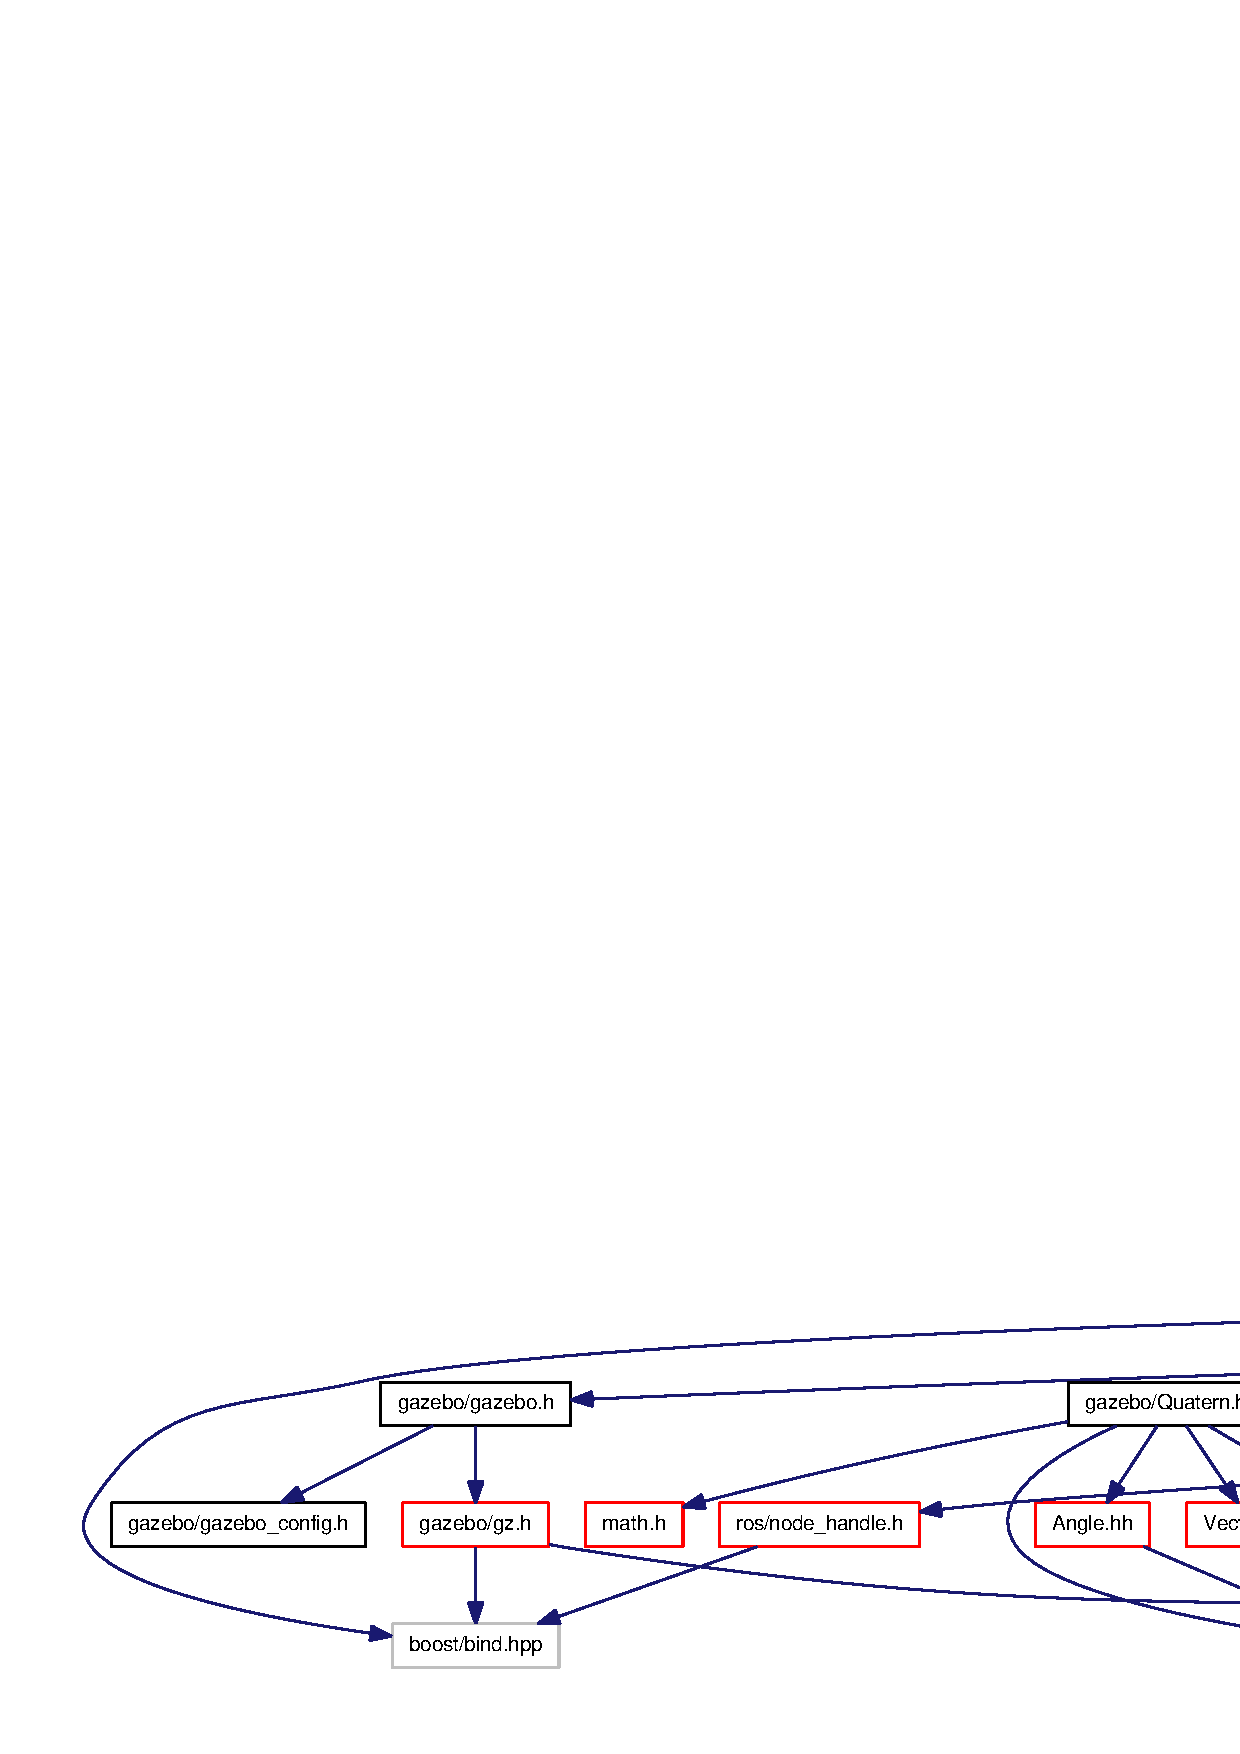
\includegraphics[width=400pt]{gazebo__ros__diffdrive_8cpp__incl}
\end{center}
\end{figure}
\subsection*{Classes}
\begin{DoxyCompactItemize}
\item 
class {\bf DiffDrive}
\end{DoxyCompactItemize}
\subsection*{Defines}
\begin{DoxyCompactItemize}
\item 
\#define {\bf DEFAULT\_\-COMMAND\_\-QUEUE}~100
\item 
\#define {\bf DEFAULT\_\-COMMAND\_\-TOPIC}~\char`\"{}cmd\_\-vel\char`\"{}
\item 
\#define {\bf DEFAULT\_\-INTERFACE\_\-NAME}~\char`\"{}position\_\-iface\_\-0\char`\"{}
\item 
\#define {\bf DEFAULT\_\-MODEL\_\-NAME}~\char`\"{}robot\_\-description\char`\"{}
\item 
\#define {\bf DEFAULT\_\-ODOMETRY\_\-QUEUE}~1
\item 
\#define {\bf DEFAULT\_\-ODOMETRY\_\-TOPIC}~\char`\"{}odom\char`\"{}
\item 
\#define {\bf DEFAULT\_\-SERVER\_\-ID}~0
\item 
\#define {\bf DEFAULT\_\-TF\_\-CHILD}~\char`\"{}base\_\-link\char`\"{}
\item 
\#define {\bf DEFAULT\_\-TF\_\-PARENT}~\char`\"{}tf\_\-parent\char`\"{}
\item 
\#define {\bf DEFAULT\_\-THREADS}~2
\item 
\#define {\bf DEFAULT\_\-UPDATE\_\-PERIOD}~0.01
\item 
\#define {\bf KEY\_\-COMMAND\_\-QUEUE}~\char`\"{}command\_\-queue\char`\"{}
\item 
\#define {\bf KEY\_\-COMMAND\_\-TOPIC}~\char`\"{}command\_\-topic\char`\"{}
\item 
\#define {\bf KEY\_\-INTERFACE\_\-NAME}~\char`\"{}interface\_\-name\char`\"{}
\item 
\#define {\bf KEY\_\-MODEL\_\-NAME}~\char`\"{}model\_\-name\char`\"{}
\item 
\#define {\bf KEY\_\-ODOMETRY\_\-QUEUE}~\char`\"{}odometry\_\-queue\char`\"{}
\item 
\#define {\bf KEY\_\-ODOMETRY\_\-TOPIC}~\char`\"{}odometry\_\-topic\char`\"{}
\item 
\#define {\bf KEY\_\-SERVER\_\-ID}~\char`\"{}server\_\-id\char`\"{}
\item 
\#define {\bf KEY\_\-TF\_\-CHILD}~\char`\"{}tf\_\-child\char`\"{}
\item 
\#define {\bf KEY\_\-TF\_\-PARENT}~\char`\"{}tf\_\-parent\char`\"{}
\item 
\#define {\bf KEY\_\-THREADS}~\char`\"{}threads\char`\"{}
\item 
\#define {\bf KEY\_\-UPDATE\_\-PERIOD}~\char`\"{}update\_\-period\char`\"{}
\end{DoxyCompactItemize}
\subsection*{Functions}
\begin{DoxyCompactItemize}
\item 
int {\bf main} (int argc, char $\ast$$\ast$argv)
\end{DoxyCompactItemize}


\subsection{Define Documentation}
\index{gazebo\_\-ros\_\-diffdrive.cpp@{gazebo\_\-ros\_\-diffdrive.cpp}!DEFAULT\_\-COMMAND\_\-QUEUE@{DEFAULT\_\-COMMAND\_\-QUEUE}}
\index{DEFAULT\_\-COMMAND\_\-QUEUE@{DEFAULT\_\-COMMAND\_\-QUEUE}!gazebo_ros_diffdrive.cpp@{gazebo\_\-ros\_\-diffdrive.cpp}}
\subsubsection[{DEFAULT\_\-COMMAND\_\-QUEUE}]{\setlength{\rightskip}{0pt plus 5cm}\#define DEFAULT\_\-COMMAND\_\-QUEUE~100}\label{gazebo__ros__diffdrive_8cpp_a68ffe50743a7896867ca4a7d01092525}


Definition at line 52 of file gazebo\_\-ros\_\-diffdrive.cpp.

\index{gazebo\_\-ros\_\-diffdrive.cpp@{gazebo\_\-ros\_\-diffdrive.cpp}!DEFAULT\_\-COMMAND\_\-TOPIC@{DEFAULT\_\-COMMAND\_\-TOPIC}}
\index{DEFAULT\_\-COMMAND\_\-TOPIC@{DEFAULT\_\-COMMAND\_\-TOPIC}!gazebo_ros_diffdrive.cpp@{gazebo\_\-ros\_\-diffdrive.cpp}}
\subsubsection[{DEFAULT\_\-COMMAND\_\-TOPIC}]{\setlength{\rightskip}{0pt plus 5cm}\#define DEFAULT\_\-COMMAND\_\-TOPIC~\char`\"{}cmd\_\-vel\char`\"{}}\label{gazebo__ros__diffdrive_8cpp_a88ab198012ad9fd21bc254626b7e297e}


Definition at line 48 of file gazebo\_\-ros\_\-diffdrive.cpp.

\index{gazebo\_\-ros\_\-diffdrive.cpp@{gazebo\_\-ros\_\-diffdrive.cpp}!DEFAULT\_\-INTERFACE\_\-NAME@{DEFAULT\_\-INTERFACE\_\-NAME}}
\index{DEFAULT\_\-INTERFACE\_\-NAME@{DEFAULT\_\-INTERFACE\_\-NAME}!gazebo_ros_diffdrive.cpp@{gazebo\_\-ros\_\-diffdrive.cpp}}
\subsubsection[{DEFAULT\_\-INTERFACE\_\-NAME}]{\setlength{\rightskip}{0pt plus 5cm}\#define DEFAULT\_\-INTERFACE\_\-NAME~\char`\"{}position\_\-iface\_\-0\char`\"{}}\label{gazebo__ros__diffdrive_8cpp_ab516f99d9b5027619fabda9c05892c15}


Definition at line 56 of file gazebo\_\-ros\_\-diffdrive.cpp.

\index{gazebo\_\-ros\_\-diffdrive.cpp@{gazebo\_\-ros\_\-diffdrive.cpp}!DEFAULT\_\-MODEL\_\-NAME@{DEFAULT\_\-MODEL\_\-NAME}}
\index{DEFAULT\_\-MODEL\_\-NAME@{DEFAULT\_\-MODEL\_\-NAME}!gazebo_ros_diffdrive.cpp@{gazebo\_\-ros\_\-diffdrive.cpp}}
\subsubsection[{DEFAULT\_\-MODEL\_\-NAME}]{\setlength{\rightskip}{0pt plus 5cm}\#define DEFAULT\_\-MODEL\_\-NAME~\char`\"{}robot\_\-description\char`\"{}}\label{gazebo__ros__diffdrive_8cpp_a39d0c3d0b96288cd4997549cc3ecc4d9}


Definition at line 55 of file gazebo\_\-ros\_\-diffdrive.cpp.

\index{gazebo\_\-ros\_\-diffdrive.cpp@{gazebo\_\-ros\_\-diffdrive.cpp}!DEFAULT\_\-ODOMETRY\_\-QUEUE@{DEFAULT\_\-ODOMETRY\_\-QUEUE}}
\index{DEFAULT\_\-ODOMETRY\_\-QUEUE@{DEFAULT\_\-ODOMETRY\_\-QUEUE}!gazebo_ros_diffdrive.cpp@{gazebo\_\-ros\_\-diffdrive.cpp}}
\subsubsection[{DEFAULT\_\-ODOMETRY\_\-QUEUE}]{\setlength{\rightskip}{0pt plus 5cm}\#define DEFAULT\_\-ODOMETRY\_\-QUEUE~1}\label{gazebo__ros__diffdrive_8cpp_a858ff692b175cfa1b91f84b0d584b20f}


Definition at line 53 of file gazebo\_\-ros\_\-diffdrive.cpp.

\index{gazebo\_\-ros\_\-diffdrive.cpp@{gazebo\_\-ros\_\-diffdrive.cpp}!DEFAULT\_\-ODOMETRY\_\-TOPIC@{DEFAULT\_\-ODOMETRY\_\-TOPIC}}
\index{DEFAULT\_\-ODOMETRY\_\-TOPIC@{DEFAULT\_\-ODOMETRY\_\-TOPIC}!gazebo_ros_diffdrive.cpp@{gazebo\_\-ros\_\-diffdrive.cpp}}
\subsubsection[{DEFAULT\_\-ODOMETRY\_\-TOPIC}]{\setlength{\rightskip}{0pt plus 5cm}\#define DEFAULT\_\-ODOMETRY\_\-TOPIC~\char`\"{}odom\char`\"{}}\label{gazebo__ros__diffdrive_8cpp_a337c1c3b23ddfadf297ae17f4dc93e1f}


Definition at line 49 of file gazebo\_\-ros\_\-diffdrive.cpp.

\index{gazebo\_\-ros\_\-diffdrive.cpp@{gazebo\_\-ros\_\-diffdrive.cpp}!DEFAULT\_\-SERVER\_\-ID@{DEFAULT\_\-SERVER\_\-ID}}
\index{DEFAULT\_\-SERVER\_\-ID@{DEFAULT\_\-SERVER\_\-ID}!gazebo_ros_diffdrive.cpp@{gazebo\_\-ros\_\-diffdrive.cpp}}
\subsubsection[{DEFAULT\_\-SERVER\_\-ID}]{\setlength{\rightskip}{0pt plus 5cm}\#define DEFAULT\_\-SERVER\_\-ID~0}\label{gazebo__ros__diffdrive_8cpp_a0ff9a709a4374667951fb31163003661}


Definition at line 50 of file gazebo\_\-ros\_\-diffdrive.cpp.

\index{gazebo\_\-ros\_\-diffdrive.cpp@{gazebo\_\-ros\_\-diffdrive.cpp}!DEFAULT\_\-TF\_\-CHILD@{DEFAULT\_\-TF\_\-CHILD}}
\index{DEFAULT\_\-TF\_\-CHILD@{DEFAULT\_\-TF\_\-CHILD}!gazebo_ros_diffdrive.cpp@{gazebo\_\-ros\_\-diffdrive.cpp}}
\subsubsection[{DEFAULT\_\-TF\_\-CHILD}]{\setlength{\rightskip}{0pt plus 5cm}\#define DEFAULT\_\-TF\_\-CHILD~\char`\"{}base\_\-link\char`\"{}}\label{gazebo__ros__diffdrive_8cpp_a0358705c8694284d288f0187e0d011c4}


Definition at line 58 of file gazebo\_\-ros\_\-diffdrive.cpp.

\index{gazebo\_\-ros\_\-diffdrive.cpp@{gazebo\_\-ros\_\-diffdrive.cpp}!DEFAULT\_\-TF\_\-PARENT@{DEFAULT\_\-TF\_\-PARENT}}
\index{DEFAULT\_\-TF\_\-PARENT@{DEFAULT\_\-TF\_\-PARENT}!gazebo_ros_diffdrive.cpp@{gazebo\_\-ros\_\-diffdrive.cpp}}
\subsubsection[{DEFAULT\_\-TF\_\-PARENT}]{\setlength{\rightskip}{0pt plus 5cm}\#define DEFAULT\_\-TF\_\-PARENT~\char`\"{}tf\_\-parent\char`\"{}}\label{gazebo__ros__diffdrive_8cpp_a5b1a3d3c086515db97209ceaafa98159}


Definition at line 57 of file gazebo\_\-ros\_\-diffdrive.cpp.

\index{gazebo\_\-ros\_\-diffdrive.cpp@{gazebo\_\-ros\_\-diffdrive.cpp}!DEFAULT\_\-THREADS@{DEFAULT\_\-THREADS}}
\index{DEFAULT\_\-THREADS@{DEFAULT\_\-THREADS}!gazebo_ros_diffdrive.cpp@{gazebo\_\-ros\_\-diffdrive.cpp}}
\subsubsection[{DEFAULT\_\-THREADS}]{\setlength{\rightskip}{0pt plus 5cm}\#define DEFAULT\_\-THREADS~2}\label{gazebo__ros__diffdrive_8cpp_af3f16d9b8a1ac1802eea6524155052c9}


Definition at line 51 of file gazebo\_\-ros\_\-diffdrive.cpp.

\index{gazebo\_\-ros\_\-diffdrive.cpp@{gazebo\_\-ros\_\-diffdrive.cpp}!DEFAULT\_\-UPDATE\_\-PERIOD@{DEFAULT\_\-UPDATE\_\-PERIOD}}
\index{DEFAULT\_\-UPDATE\_\-PERIOD@{DEFAULT\_\-UPDATE\_\-PERIOD}!gazebo_ros_diffdrive.cpp@{gazebo\_\-ros\_\-diffdrive.cpp}}
\subsubsection[{DEFAULT\_\-UPDATE\_\-PERIOD}]{\setlength{\rightskip}{0pt plus 5cm}\#define DEFAULT\_\-UPDATE\_\-PERIOD~0.01}\label{gazebo__ros__diffdrive_8cpp_a9064e22b01bc8ae3350cefd103a4a2dc}


Definition at line 54 of file gazebo\_\-ros\_\-diffdrive.cpp.

\index{gazebo\_\-ros\_\-diffdrive.cpp@{gazebo\_\-ros\_\-diffdrive.cpp}!KEY\_\-COMMAND\_\-QUEUE@{KEY\_\-COMMAND\_\-QUEUE}}
\index{KEY\_\-COMMAND\_\-QUEUE@{KEY\_\-COMMAND\_\-QUEUE}!gazebo_ros_diffdrive.cpp@{gazebo\_\-ros\_\-diffdrive.cpp}}
\subsubsection[{KEY\_\-COMMAND\_\-QUEUE}]{\setlength{\rightskip}{0pt plus 5cm}\#define KEY\_\-COMMAND\_\-QUEUE~\char`\"{}command\_\-queue\char`\"{}}\label{gazebo__ros__diffdrive_8cpp_adae44ae0588dd90ab5f114337933004e}


Definition at line 40 of file gazebo\_\-ros\_\-diffdrive.cpp.

\index{gazebo\_\-ros\_\-diffdrive.cpp@{gazebo\_\-ros\_\-diffdrive.cpp}!KEY\_\-COMMAND\_\-TOPIC@{KEY\_\-COMMAND\_\-TOPIC}}
\index{KEY\_\-COMMAND\_\-TOPIC@{KEY\_\-COMMAND\_\-TOPIC}!gazebo_ros_diffdrive.cpp@{gazebo\_\-ros\_\-diffdrive.cpp}}
\subsubsection[{KEY\_\-COMMAND\_\-TOPIC}]{\setlength{\rightskip}{0pt plus 5cm}\#define KEY\_\-COMMAND\_\-TOPIC~\char`\"{}command\_\-topic\char`\"{}}\label{gazebo__ros__diffdrive_8cpp_abf7a2dd6a4db4df02ec95dacaf116122}


Definition at line 36 of file gazebo\_\-ros\_\-diffdrive.cpp.

\index{gazebo\_\-ros\_\-diffdrive.cpp@{gazebo\_\-ros\_\-diffdrive.cpp}!KEY\_\-INTERFACE\_\-NAME@{KEY\_\-INTERFACE\_\-NAME}}
\index{KEY\_\-INTERFACE\_\-NAME@{KEY\_\-INTERFACE\_\-NAME}!gazebo_ros_diffdrive.cpp@{gazebo\_\-ros\_\-diffdrive.cpp}}
\subsubsection[{KEY\_\-INTERFACE\_\-NAME}]{\setlength{\rightskip}{0pt plus 5cm}\#define KEY\_\-INTERFACE\_\-NAME~\char`\"{}interface\_\-name\char`\"{}}\label{gazebo__ros__diffdrive_8cpp_a507d0de0321d431dbef9e235cf1c222f}


Definition at line 44 of file gazebo\_\-ros\_\-diffdrive.cpp.

\index{gazebo\_\-ros\_\-diffdrive.cpp@{gazebo\_\-ros\_\-diffdrive.cpp}!KEY\_\-MODEL\_\-NAME@{KEY\_\-MODEL\_\-NAME}}
\index{KEY\_\-MODEL\_\-NAME@{KEY\_\-MODEL\_\-NAME}!gazebo_ros_diffdrive.cpp@{gazebo\_\-ros\_\-diffdrive.cpp}}
\subsubsection[{KEY\_\-MODEL\_\-NAME}]{\setlength{\rightskip}{0pt plus 5cm}\#define KEY\_\-MODEL\_\-NAME~\char`\"{}model\_\-name\char`\"{}}\label{gazebo__ros__diffdrive_8cpp_a2c53a2fc3c18baa21d5871179ae085a8}


Definition at line 43 of file gazebo\_\-ros\_\-diffdrive.cpp.

\index{gazebo\_\-ros\_\-diffdrive.cpp@{gazebo\_\-ros\_\-diffdrive.cpp}!KEY\_\-ODOMETRY\_\-QUEUE@{KEY\_\-ODOMETRY\_\-QUEUE}}
\index{KEY\_\-ODOMETRY\_\-QUEUE@{KEY\_\-ODOMETRY\_\-QUEUE}!gazebo_ros_diffdrive.cpp@{gazebo\_\-ros\_\-diffdrive.cpp}}
\subsubsection[{KEY\_\-ODOMETRY\_\-QUEUE}]{\setlength{\rightskip}{0pt plus 5cm}\#define KEY\_\-ODOMETRY\_\-QUEUE~\char`\"{}odometry\_\-queue\char`\"{}}\label{gazebo__ros__diffdrive_8cpp_a0ec020516db9e7a344c908eff44e743d}


Definition at line 41 of file gazebo\_\-ros\_\-diffdrive.cpp.

\index{gazebo\_\-ros\_\-diffdrive.cpp@{gazebo\_\-ros\_\-diffdrive.cpp}!KEY\_\-ODOMETRY\_\-TOPIC@{KEY\_\-ODOMETRY\_\-TOPIC}}
\index{KEY\_\-ODOMETRY\_\-TOPIC@{KEY\_\-ODOMETRY\_\-TOPIC}!gazebo_ros_diffdrive.cpp@{gazebo\_\-ros\_\-diffdrive.cpp}}
\subsubsection[{KEY\_\-ODOMETRY\_\-TOPIC}]{\setlength{\rightskip}{0pt plus 5cm}\#define KEY\_\-ODOMETRY\_\-TOPIC~\char`\"{}odometry\_\-topic\char`\"{}}\label{gazebo__ros__diffdrive_8cpp_ab75ee4b79a80a1bd5262af8bbad37d04}


Definition at line 37 of file gazebo\_\-ros\_\-diffdrive.cpp.

\index{gazebo\_\-ros\_\-diffdrive.cpp@{gazebo\_\-ros\_\-diffdrive.cpp}!KEY\_\-SERVER\_\-ID@{KEY\_\-SERVER\_\-ID}}
\index{KEY\_\-SERVER\_\-ID@{KEY\_\-SERVER\_\-ID}!gazebo_ros_diffdrive.cpp@{gazebo\_\-ros\_\-diffdrive.cpp}}
\subsubsection[{KEY\_\-SERVER\_\-ID}]{\setlength{\rightskip}{0pt plus 5cm}\#define KEY\_\-SERVER\_\-ID~\char`\"{}server\_\-id\char`\"{}}\label{gazebo__ros__diffdrive_8cpp_aba838f74774271adc62f5223c844f0fe}


Definition at line 38 of file gazebo\_\-ros\_\-diffdrive.cpp.

\index{gazebo\_\-ros\_\-diffdrive.cpp@{gazebo\_\-ros\_\-diffdrive.cpp}!KEY\_\-TF\_\-CHILD@{KEY\_\-TF\_\-CHILD}}
\index{KEY\_\-TF\_\-CHILD@{KEY\_\-TF\_\-CHILD}!gazebo_ros_diffdrive.cpp@{gazebo\_\-ros\_\-diffdrive.cpp}}
\subsubsection[{KEY\_\-TF\_\-CHILD}]{\setlength{\rightskip}{0pt plus 5cm}\#define KEY\_\-TF\_\-CHILD~\char`\"{}tf\_\-child\char`\"{}}\label{gazebo__ros__diffdrive_8cpp_a70e360a50e857ffc6f32982ee73488f1}


Definition at line 46 of file gazebo\_\-ros\_\-diffdrive.cpp.

\index{gazebo\_\-ros\_\-diffdrive.cpp@{gazebo\_\-ros\_\-diffdrive.cpp}!KEY\_\-TF\_\-PARENT@{KEY\_\-TF\_\-PARENT}}
\index{KEY\_\-TF\_\-PARENT@{KEY\_\-TF\_\-PARENT}!gazebo_ros_diffdrive.cpp@{gazebo\_\-ros\_\-diffdrive.cpp}}
\subsubsection[{KEY\_\-TF\_\-PARENT}]{\setlength{\rightskip}{0pt plus 5cm}\#define KEY\_\-TF\_\-PARENT~\char`\"{}tf\_\-parent\char`\"{}}\label{gazebo__ros__diffdrive_8cpp_a526b0d72a46fac5e090caf049c1bb2ac}


Definition at line 45 of file gazebo\_\-ros\_\-diffdrive.cpp.

\index{gazebo\_\-ros\_\-diffdrive.cpp@{gazebo\_\-ros\_\-diffdrive.cpp}!KEY\_\-THREADS@{KEY\_\-THREADS}}
\index{KEY\_\-THREADS@{KEY\_\-THREADS}!gazebo_ros_diffdrive.cpp@{gazebo\_\-ros\_\-diffdrive.cpp}}
\subsubsection[{KEY\_\-THREADS}]{\setlength{\rightskip}{0pt plus 5cm}\#define KEY\_\-THREADS~\char`\"{}threads\char`\"{}}\label{gazebo__ros__diffdrive_8cpp_a1c0b253edf7ef5e6eaf91e33c729947e}


Definition at line 39 of file gazebo\_\-ros\_\-diffdrive.cpp.

\index{gazebo\_\-ros\_\-diffdrive.cpp@{gazebo\_\-ros\_\-diffdrive.cpp}!KEY\_\-UPDATE\_\-PERIOD@{KEY\_\-UPDATE\_\-PERIOD}}
\index{KEY\_\-UPDATE\_\-PERIOD@{KEY\_\-UPDATE\_\-PERIOD}!gazebo_ros_diffdrive.cpp@{gazebo\_\-ros\_\-diffdrive.cpp}}
\subsubsection[{KEY\_\-UPDATE\_\-PERIOD}]{\setlength{\rightskip}{0pt plus 5cm}\#define KEY\_\-UPDATE\_\-PERIOD~\char`\"{}update\_\-period\char`\"{}}\label{gazebo__ros__diffdrive_8cpp_a86e39a07c79ab4ac9750a5c7fae16b3d}


Definition at line 42 of file gazebo\_\-ros\_\-diffdrive.cpp.



\subsection{Function Documentation}
\index{gazebo\_\-ros\_\-diffdrive.cpp@{gazebo\_\-ros\_\-diffdrive.cpp}!main@{main}}
\index{main@{main}!gazebo_ros_diffdrive.cpp@{gazebo\_\-ros\_\-diffdrive.cpp}}
\subsubsection[{main}]{\setlength{\rightskip}{0pt plus 5cm}int main (
\begin{DoxyParamCaption}
\item[{int}]{argc, }
\item[{char $\ast$$\ast$}]{argv}
\end{DoxyParamCaption}
)}\label{gazebo__ros__diffdrive_8cpp_a3c04138a5bfe5d72780bb7e82a18e627}


Definition at line 239 of file gazebo\_\-ros\_\-diffdrive.cpp.


\section{/home/klc/Code/github.com/my\_\-stack/my\_\-gazebo\_\-drivers/src/gazebo\_\-ros\_\-diffdrive\_\-plugin.cpp File Reference}
\label{gazebo__ros__diffdrive__plugin_8cpp}\index{/home/klc/Code/github.com/my\_\-stack/my\_\-gazebo\_\-drivers/src/gazebo\_\-ros\_\-diffdrive\_\-plugin.cpp@{/home/klc/Code/github.com/my\_\-stack/my\_\-gazebo\_\-drivers/src/gazebo\_\-ros\_\-diffdrive\_\-plugin.cpp}}
{\ttfamily \#include $<$map$>$}\par
{\ttfamily \#include $<$gazebo/Param.hh$>$}\par
{\ttfamily \#include $<$gazebo/Controller.hh$>$}\par
{\ttfamily \#include $<$gazebo/Model.hh$>$}\par
{\ttfamily \#include $<$ros/ros.h$>$}\par
{\ttfamily \#include $<$tf/transform\_\-broadcaster.h$>$}\par
{\ttfamily \#include $<$tf/transform\_\-listener.h$>$}\par
{\ttfamily \#include $<$geometry\_\-msgs/Twist.h$>$}\par
{\ttfamily \#include $<$nav\_\-msgs/Odometry.h$>$}\par
{\ttfamily \#include $<$ros/callback\_\-queue.h$>$}\par
{\ttfamily \#include $<$ros/advertise\_\-options.h$>$}\par
{\ttfamily \#include $<$boost/thread.hpp$>$}\par
{\ttfamily \#include $<$boost/bind.hpp$>$}\par
{\ttfamily \#include $<$algorithm$>$}\par
{\ttfamily \#include $<$assert.h$>$}\par
{\ttfamily \#include $<$gazebo/gazebo.h$>$}\par
{\ttfamily \#include $<$gazebo/GazeboError.hh$>$}\par
{\ttfamily \#include $<$gazebo/Quatern.hh$>$}\par
{\ttfamily \#include $<$gazebo/Body.hh$>$}\par
{\ttfamily \#include $<$gazebo/World.hh$>$}\par
{\ttfamily \#include $<$gazebo/Simulator.hh$>$}\par
{\ttfamily \#include $<$gazebo/Global.hh$>$}\par
{\ttfamily \#include $<$gazebo/XMLConfig.hh$>$}\par
{\ttfamily \#include $<$gazebo/ControllerFactory.hh$>$}\par
{\ttfamily \#include $<$gazebo/PhysicsEngine.hh$>$}\par
Include dependency graph for gazebo\_\-ros\_\-diffdrive\_\-plugin.cpp:
\nopagebreak
\begin{figure}[H]
\begin{center}
\leavevmode
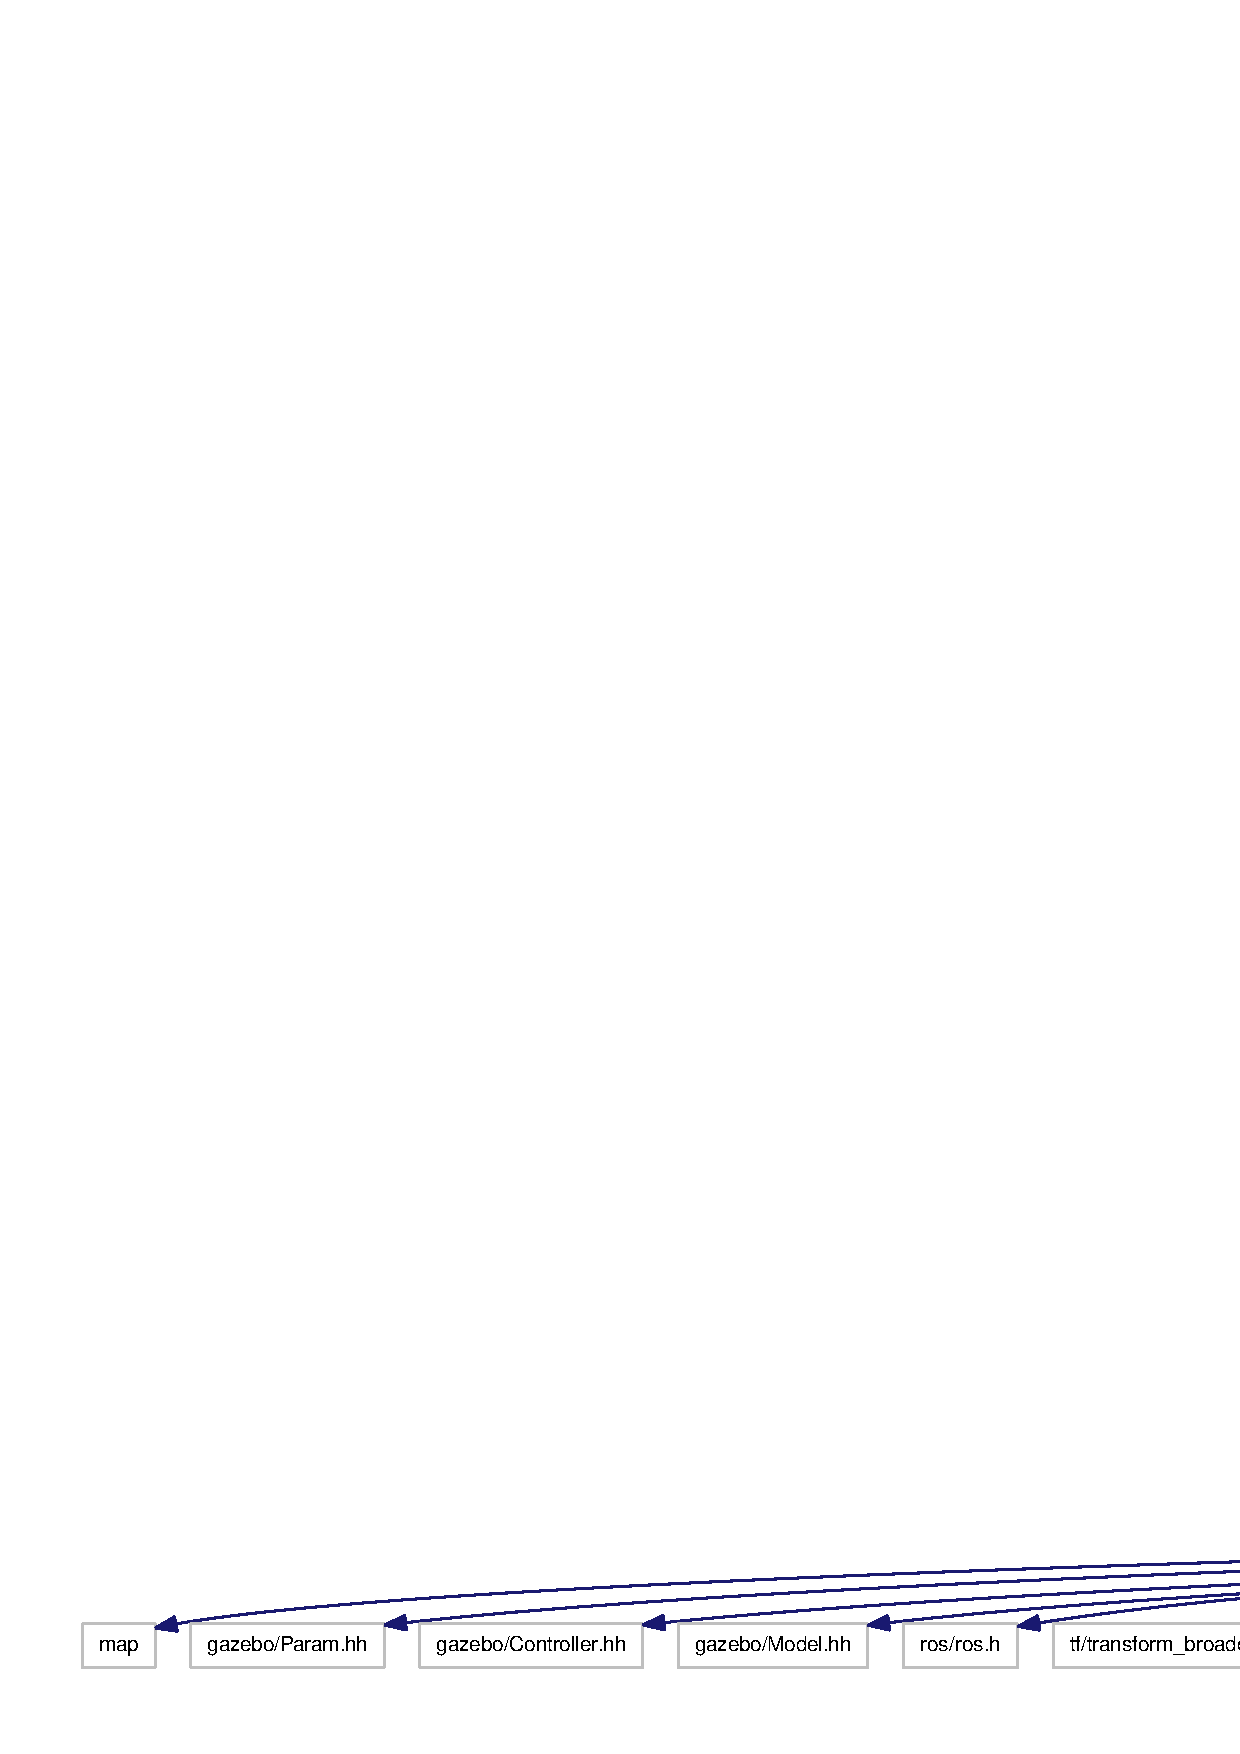
\includegraphics[width=400pt]{gazebo__ros__diffdrive__plugin_8cpp__incl}
\end{center}
\end{figure}
\subsection*{Classes}
\begin{DoxyCompactItemize}
\item 
class {\bf gazebo::DiffDrivePlugin}
\end{DoxyCompactItemize}
\subsection*{Namespaces}
\begin{DoxyCompactItemize}
\item 
namespace {\bf gazebo}
\end{DoxyCompactItemize}
\subsection*{Enumerations}
\begin{DoxyCompactItemize}
\item 
enum \{ {\bf RIGHT}, 
{\bf LEFT}
 \}
\end{DoxyCompactItemize}
\subsection*{Functions}
\begin{DoxyCompactItemize}
\item 
{\bf GZ\_\-REGISTER\_\-DYNAMIC\_\-CONTROLLER} (\char`\"{}gazebo\_\-ros\_\-diffdrive\_\-plugin\char`\"{}, DiffDrivePlugin)
\end{DoxyCompactItemize}


\subsection{Enumeration Type Documentation}
\subsubsection[{"@0}]{\setlength{\rightskip}{0pt plus 5cm}anonymous enum}\label{gazebo__ros__diffdrive__plugin_8cpp_a06fc87d81c62e9abb8790b6e5713c55b}
\begin{Desc}
\item[Enumerator: ]\par
\begin{description}
\index{RIGHT@{RIGHT}!gazebo\_\-ros\_\-diffdrive\_\-plugin.cpp@{gazebo\_\-ros\_\-diffdrive\_\-plugin.cpp}}\index{gazebo\_\-ros\_\-diffdrive\_\-plugin.cpp@{gazebo\_\-ros\_\-diffdrive\_\-plugin.cpp}!RIGHT@{RIGHT}}\item[{\em 
RIGHT\label{gazebo__ros__diffdrive__plugin_8cpp_a06fc87d81c62e9abb8790b6e5713c55baec8379af7490bb9eaaf579cf17876f38}
}]\index{LEFT@{LEFT}!gazebo\_\-ros\_\-diffdrive\_\-plugin.cpp@{gazebo\_\-ros\_\-diffdrive\_\-plugin.cpp}}\index{gazebo\_\-ros\_\-diffdrive\_\-plugin.cpp@{gazebo\_\-ros\_\-diffdrive\_\-plugin.cpp}!LEFT@{LEFT}}\item[{\em 
LEFT\label{gazebo__ros__diffdrive__plugin_8cpp_a06fc87d81c62e9abb8790b6e5713c55badb45120aafd37a973140edee24708065}
}]\end{description}
\end{Desc}



Definition at line 172 of file gazebo\_\-ros\_\-diffdrive\_\-plugin.cpp.



\subsection{Function Documentation}
\index{gazebo\_\-ros\_\-diffdrive\_\-plugin.cpp@{gazebo\_\-ros\_\-diffdrive\_\-plugin.cpp}!GZ\_\-REGISTER\_\-DYNAMIC\_\-CONTROLLER@{GZ\_\-REGISTER\_\-DYNAMIC\_\-CONTROLLER}}
\index{GZ\_\-REGISTER\_\-DYNAMIC\_\-CONTROLLER@{GZ\_\-REGISTER\_\-DYNAMIC\_\-CONTROLLER}!gazebo_ros_diffdrive_plugin.cpp@{gazebo\_\-ros\_\-diffdrive\_\-plugin.cpp}}
\subsubsection[{GZ\_\-REGISTER\_\-DYNAMIC\_\-CONTROLLER}]{\setlength{\rightskip}{0pt plus 5cm}GZ\_\-REGISTER\_\-DYNAMIC\_\-CONTROLLER (
\begin{DoxyParamCaption}
\item[{\char`\"{}gazebo\_\-ros\_\-diffdrive\_\-plugin\char`\"{}}]{, }
\item[{{\bf DiffDrivePlugin}}]{}
\end{DoxyParamCaption}
)}\label{gazebo__ros__diffdrive__plugin_8cpp_a29c0cb7a93e10a50fcf40774efed423d}

\printindex
\end{document}
